% The four ROS 2 nodes and the topics between them (node code in ros2_ws/src). Solid: this repository; dashed: existing package;
% grey: hardware. Orange: a track direction projected into the camera image and matched to a face within 20 degrees.
\documentclass[border=1.5pt]{standalone}
% Shared look of the figures in docs/. Text 8 pt, Times.
% Colors: cInk for this device's code and data, cFace (grey fill) for hardware, cCal for the one point each figure is about.
\usepackage[T1]{fontenc}
\usepackage{times}
\usepackage{amsmath,amssymb}
\usepackage{xcolor}
\usepackage{tikz}
\usepackage{pgfplots,pgfplotstable}
\pgfplotsset{compat=1.18}
\usetikzlibrary{arrows.meta,positioning,calc}
\usepgfplotslibrary{groupplots}

\definecolor{cCal}{HTML}{D55E00}
\definecolor{cInk}{HTML}{1F2933}
\definecolor{cMuted}{HTML}{6B7280}
\definecolor{cGrid}{HTML}{E3E6EA}
\color{cInk}

\newcommand{\figfont}{\fontsize{8}{9.5}\selectfont}
\newcommand{\figsmall}{\fontsize{8}{9.5}\selectfont}

\pgfplotsset{
  spl/.style={
    width=44mm, height=36mm, scale only axis=false,
    axis line style={cMuted, line width=0.5pt},
    tick style={cMuted, line width=0.5pt}, tick align=outside,
    tick label style={font=\figsmall, text=cInk},
    label style={font=\figfont, text=cInk},
    legend style={font=\figsmall, draw=none, fill=none, text=cInk, inner sep=0pt},
    legend cell align=left,
    grid=major, major grid style={cGrid, line width=0.4pt},
    axis lines*=left, clip mode=individual,
    every axis plot/.append style={line width=0.9pt},
  },
}

\definecolor{cFace}{HTML}{E2E5E9}
\begin{document}
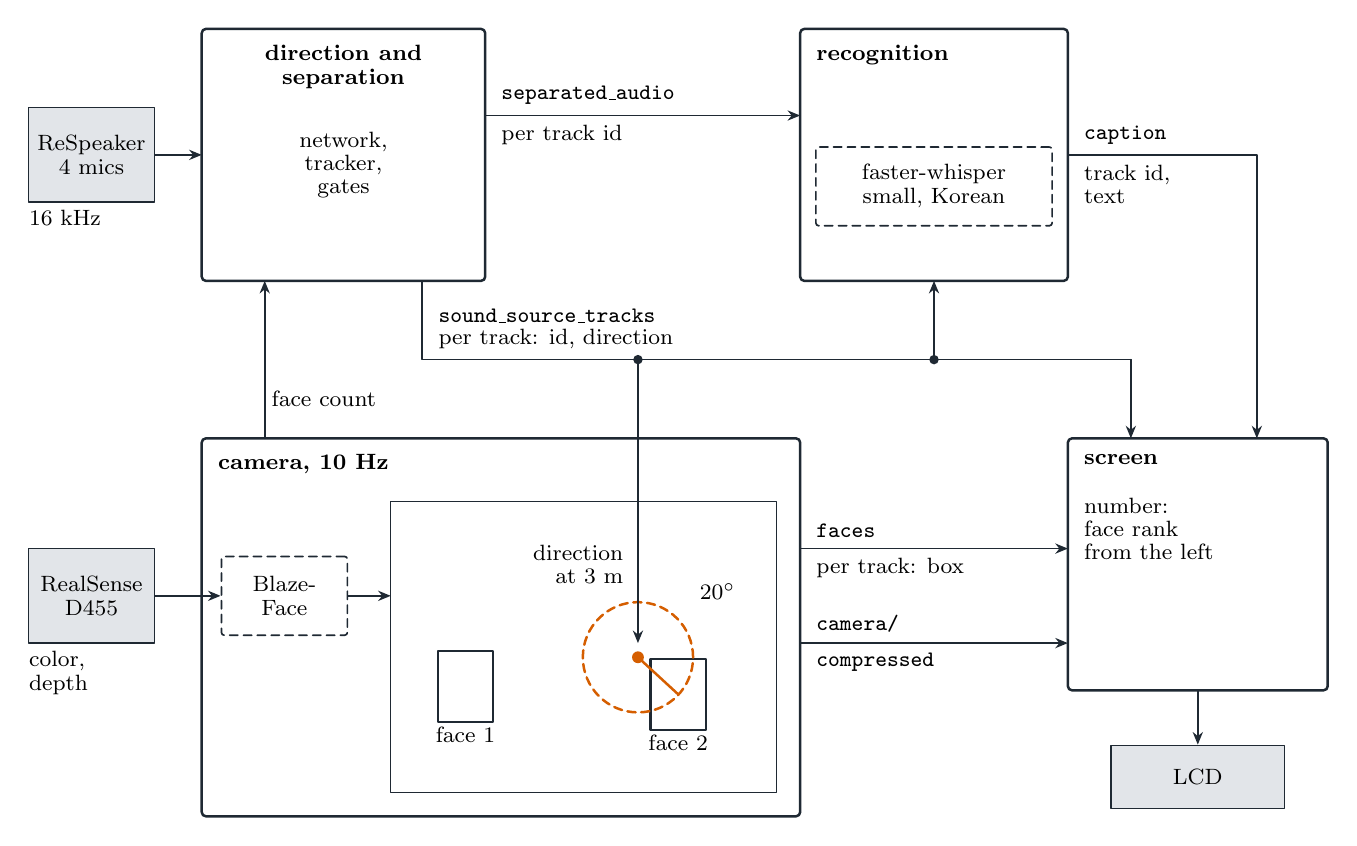
\begin{tikzpicture}[x=1mm, y=1mm, font=\figfont, line join=round, line cap=round,
  node/.style={draw=cInk, line width=0.9pt, rounded corners=1.5pt, fill=white},
  own/.style={draw=cInk, line width=0.6pt, rounded corners=1pt, align=center, inner xsep=0.8mm, inner ysep=0.8mm, fill=white, minimum height=10mm},
  pkg/.style={own, densely dashed},
  hw/.style={draw=cInk, line width=0.6pt, align=center, inner xsep=0.8mm, inner ysep=1.0mm, fill=cFace},
  flow/.style={-{Stealth[length=1.6mm, width=1.3mm]}, line width=0.6pt, draw=cInk},
  bus/.style={line width=0.6pt, draw=cInk},
  topic/.style={font=\ttfamily\bfseries\figsmall, inner sep=0pt},
  card/.style={align=left, inner sep=0pt},
  focus/.style={draw=cCal, line width=0.9pt}]

% hardware
\node[hw, minimum width=16mm, minimum height=12mm] (mic) at (8,86) {ReSpeaker\\[-0.3mm]4 mics};
\node[card, anchor=north west] at (0,79) {16 kHz};
\node[hw, minimum width=16mm, minimum height=12mm] (cam) at (8,30) {RealSense\\[-0.3mm]D455};
\node[card, anchor=north west] at (0,23) {color,\\[-0.4mm]depth};

% direction and separation
\draw[node] (22,70) rectangle (58,102);
\node[anchor=north, inner sep=0pt, align=center] at (40,100) {\textbf{direction and}\\[-0.3mm]\textbf{separation}};
\node[card, anchor=north, align=center] at (40,89) {network,\\[-0.4mm]tracker,\\[-0.4mm]gates};
\draw[flow] (mic.east) -- (22,86);

% recognition
\draw[node] (98,70) rectangle (132,102);
\node[anchor=north west, inner sep=0pt] at (100,100) {\textbf{recognition}};
\node[pkg, minimum width=30mm] at (115,82) {faster-whisper\\[-0.3mm]small, Korean};
\draw[flow] (58,91) -- (98,91);
\node[topic, anchor=south west] at (60,92.3) {separated\_audio};
\node[card, anchor=north west] at (60,89.8) {per track id};

% camera node
\draw[node] (22,2) rectangle (98,50);
\node[anchor=north west, inner sep=0pt] at (24,48) {\textbf{camera, 10 Hz}};
\node[pkg, minimum width=16mm] (bf) at (32.5,30) {Blaze-\\[-0.3mm]Face};
\draw[flow] (cam.east) -- (bf.west);
\draw[cInk, line width=0.5pt, fill=white] (46,5) rectangle (95,42);
\draw[flow] (bf.east) -- (46,30);
\draw[cInk, line width=0.8pt] (52,14) rectangle (59,23);
\draw[cInk, line width=0.8pt] (79,13) rectangle (86,22);
\node[inner sep=0.6mm, anchor=north] at (55.5,14) {face 1};
\node[inner sep=0.6mm, anchor=north] at (82.5,13) {face 2};
\fill[cCal] (77.4,22.2) circle (0.75);
\draw[focus, densely dashed] (77.4,22.2) circle (7.0);
\draw[focus] (77.4,22.2) -- (82.5,17.5);
\node[card, anchor=east, align=right] at (75.6,34.0) {direction\\[-0.4mm]at 3 m};
\node[card, anchor=west] at (85.2,30.5) {20$^\circ$};

% screen
\draw[node] (132,18) rectangle (165,50);
\node[anchor=north west, inner sep=0pt] at (134,48) {\textbf{screen}};
\node[card, anchor=north west] at (134,42.5) {number:\\[-0.4mm]face rank\\[-0.4mm]from the left};
\node[hw, minimum width=22mm, minimum height=8mm] (lcd) at (148.5,7) {LCD};
\draw[flow] (148.5,18) -- (lcd.north);

% sound_source_tracks bus
\draw[bus] (50,70) -- (50,60) -- (140,60);
\draw[flow] (77.4,60) -- (77.4,24.0);
\draw[flow] (115,60) -- (115,70);
\draw[flow] (140,60) -- (140,50);
\fill[cInk] (77.4,60) circle (0.6) (115,60) circle (0.6);
\node[topic, anchor=south west] at (52,64.6) {sound\_source\_tracks};
\node[card, anchor=north west] at (52,64.0) {per track: id, direction};

% faces back to the direction node
\draw[flow] (30,50) -- (30,70);
\node[card, anchor=west, inner sep=0.8mm] at (30,55) {face count};

% faces and image to the screen
\draw[flow] (98,36) -- (132,36);
\node[topic, anchor=south west] at (100,37.3) {faces};
\node[card, anchor=north west] at (100,34.8) {per track: box};
\draw[flow] (98,24) -- (132,24);
\node[topic, anchor=south west] at (100,25.3) {camera/};
\node[topic, anchor=north west] at (100,22.8) {compressed};

% caption
\draw[flow] (132,86) -- (156,86) -- (156,50);
\node[topic, anchor=south west] at (134,87.3) {caption};
\node[card, anchor=north west] at (134,84.8) {track id,\\[-0.4mm]text};
\end{tikzpicture}
\end{document}
